\documentclass[tikz]{standalone}
\usetikzlibrary{arrows,angles,quotes,calc}
\begin{document}
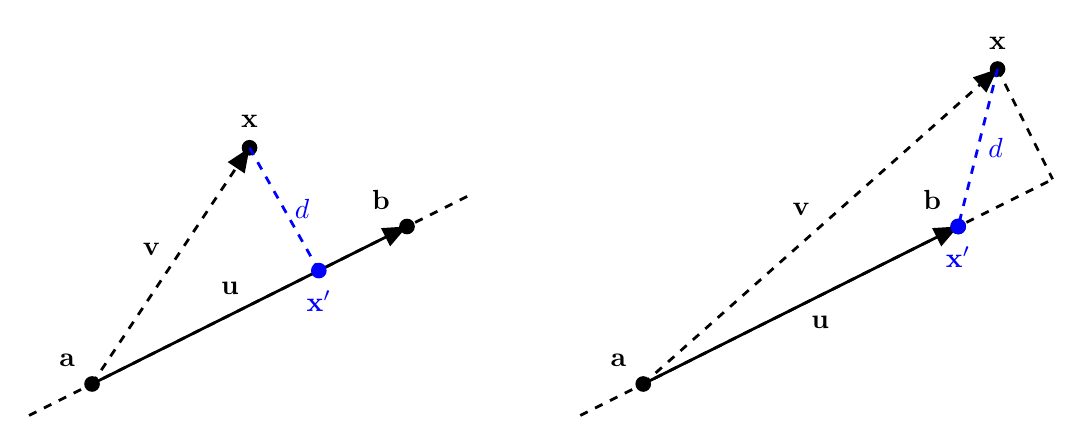
\begin{tikzpicture}[>=triangle 45,line width=1pt,scale=1.0,font=\fontsize{10pt}{0}]

\begin{scope}
  \coordinate (A) at (0,0);
  \coordinate (B) at (4,2);
  \coordinate (C) at (2,3);
  \node[fill,inner sep=2pt,circle,label=135:$\mathbf{a}$] at (A) {};
  \node[fill,inner sep=2pt,circle,label=135:$\mathbf{b}$] at (B) {};
  \node[fill,inner sep=2pt,circle,label=$\mathbf{x}$] at (C) {};
  \draw[->] (A) -- (B) node[midway, anchor=south east] {$\mathbf{u}$};
  \draw[->,dashed] (A) -- (C) node[midway, anchor=south east] {$\mathbf{v}$};
  \draw[dashed] ($(A)!-0.2!(B)$) -- ($(A)!1.2!(B)$);
  \draw[dashed, blue](C) -- ($(A)!0.72!(B)$) node[midway, anchor=west] {$d$} node[fill,inner sep=2pt,circle,label=-90:$\mathbf{x}'$] {};
\end{scope}

\begin{scope}[xshift=7cm]
  \coordinate (A) at (0,0);
  \coordinate (B) at (4,2);
  \coordinate (C) at (4.5,4);
  \node[fill,inner sep=2pt,circle,label=135:$\mathbf{a}$] at (A) {};
  \node[fill,inner sep=2pt,circle,label=135:$\mathbf{b}$] at (B) {};
  \node[fill,inner sep=2pt,circle,label=$\mathbf{x}$] at (C) {};
  \draw[->] (A) -- (B) node[midway, anchor=north west] {$\mathbf{u}$};
  \draw[->,dashed] (A) -- (C) node[midway, anchor=south east] {$\mathbf{v}$};
  \draw[dashed] ($(A)!-0.2!(B)$) -- ($(A)!1.3!(B)$);
  \draw[dashed](C) -- ($(A)!1.3!(B)$);
  \draw[dashed, blue](C) -- (B) node[midway, anchor=west] {$d$} node[fill,inner sep=2pt,circle,label=-90:$\mathbf{x}'$] {};
\end{scope}

\end{tikzpicture}
\end{document}
